%%%%%%%%%%%%
%
% $Autor: Wings $
% $Datum: 2019-03-05 08:03:15Z $
% $Pfad: TemplateSensor $
% $Version: 4250 $
% !TeX spellcheck = en_GB/de_DE
% !TeX encoding = utf8
% !TeX root = filename 
% !TeX TXS-program:bibliography = txs:///biber
%
%%%%%%%%%%%%

% Structure
\chapter{DC-Gleichstrommotor}


\section{Allgemeines}

General description

cite books

\section{Motraxx SR555SHP}

cite board

\section{Spezifikationen}

\begin{center}
	\begin{figure}
		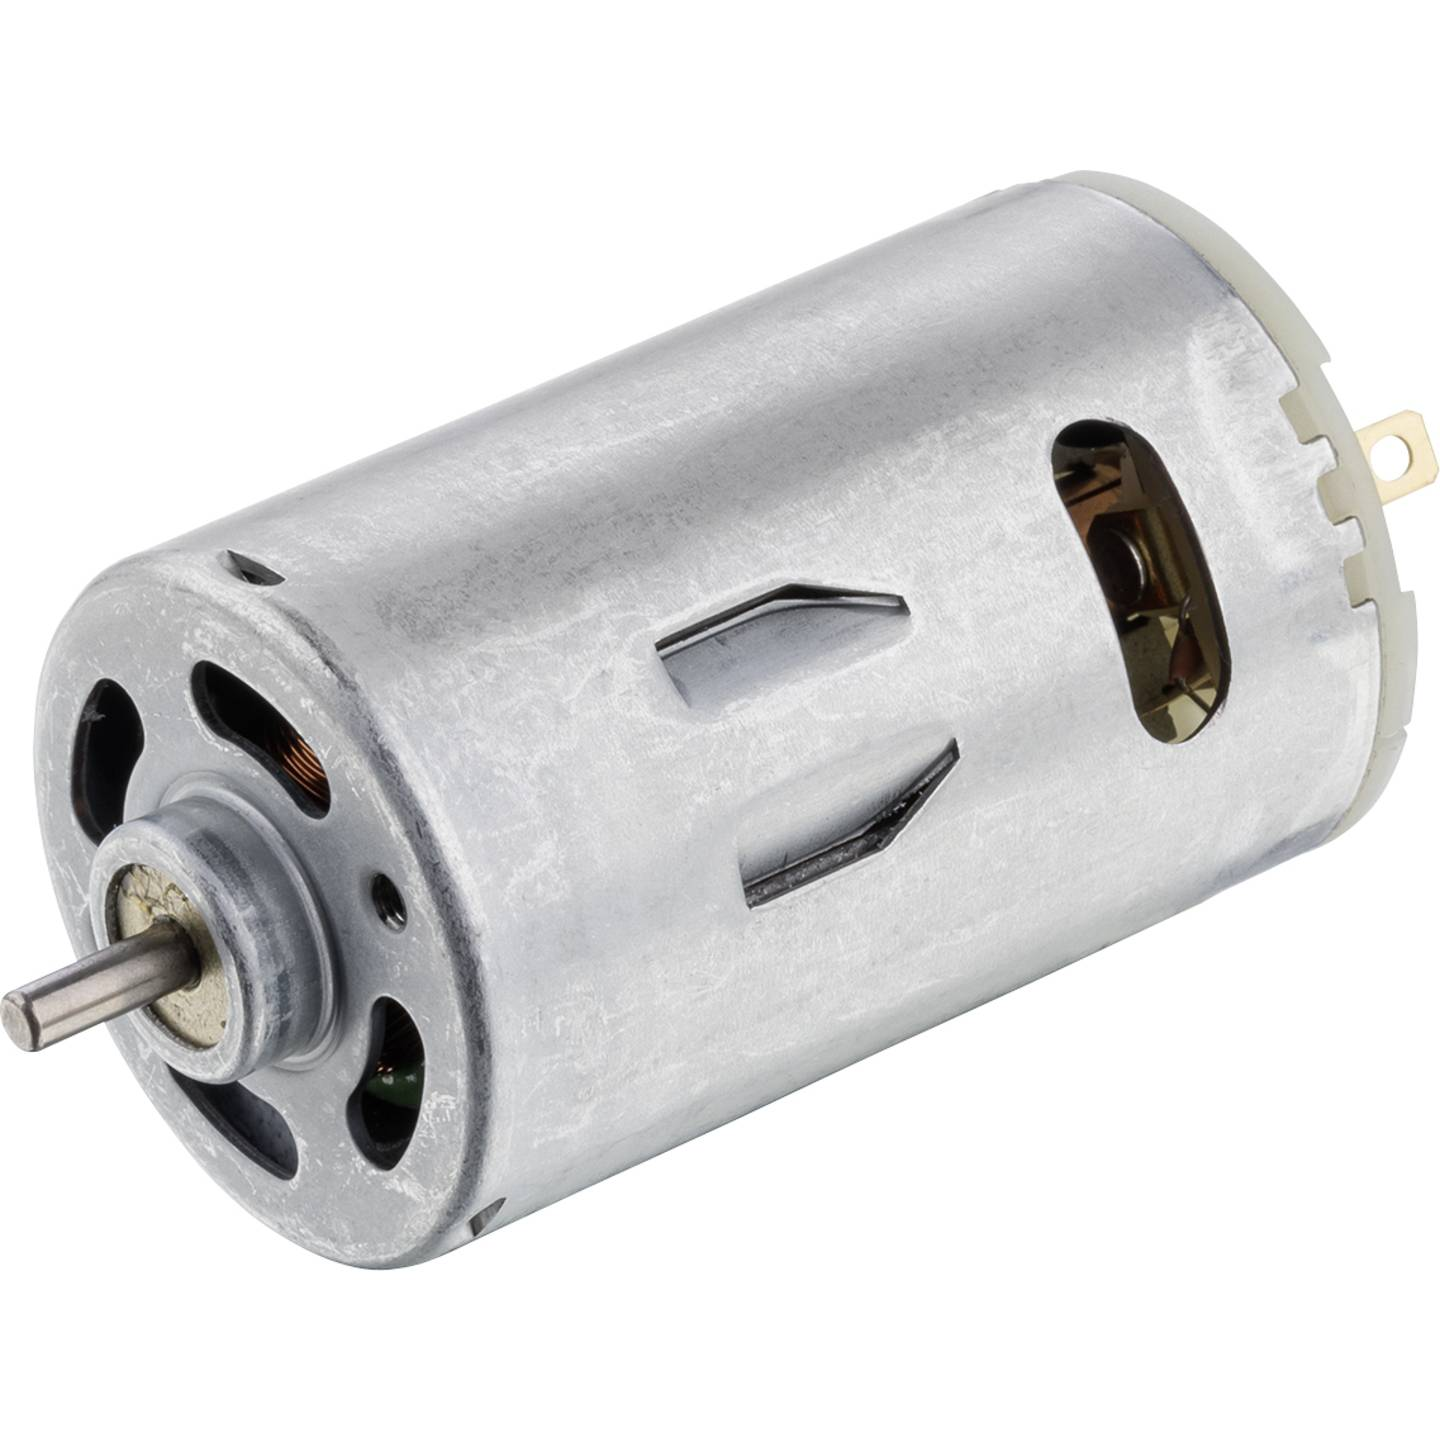
\includegraphics[scale=0.25]{../../Images/BOM/Motraxx_SR555SHP-3247S-75_Universal_Brushed_Elektromotor.jpg}
		\caption{Der Motor Motraxx SR555SHP nach (QUELLE)} 
		\label{pic:SR555SHP}
	\end{figure}
\end{center}

\begin{table}[h!]
	\caption{Spezifikationen des Motors (QUELLE)}
	\begin{center}
		\begin{tabular}{|l|l|}
			\hline
			\textbf{Parameter} &\textbf{Wert/Detail}\\
			\hline
			Modell &  SR555SHP\\
			\hline
			Typ  & DC-Gleichstrommotor\\
			\hline 
			Betriebsspannung & 10 bis 14 $V$ DC\\
			\hline 
			Nennspannung & 12 $V$ DC\\
			\hline
			Abgabeleistung & 13 $W$\\
			\hline
			Last-Drehzahl & 4800 $U/min$ \\
			\hline
			Max. Drehmoment & 25.18 $Nmm$\\
			\hline
			Anschlüsse & +V, -V\\ 
			\hline
			Wellen-Ø & 3.175 $mm$\\ 
			\hline
			Durchmesser & 37.5 $mm$\\ 
			\hline
			Länge & 57 $mm$\\ 
			\hline
			Gewicht & 224 $g$\\ 
			\hline
		\end{tabular}
		\label{TabelleSpezifikationLS}
	\end{center}
\end{table} 


Der Motortreiber besitzt wie in \ref{pic:SR555SHP} erkenntlich zwei Anschlüsse. Diese Anschlüsse können wie folgt beschrieben werden: 
\begin{enumerate}
	\item \textbf{Leistungsanschlüsse}
	\begin{itemize}
		\item \textbf{+V}: Positiver Spannungsanschluss (10$-$14 $V$ DC)
		\item \textbf{-V}: Negativer Spannungsanschluss (Masse)
	\end{itemize}
\end{enumerate}



\section{Anwendungsbeispiel}
\label{sec:AnwendungSR555SHP}
Der Motortreiber lässt sich mit kleinem Aufwand anschließen und verwenden. 
Es muss sichergestellt sein, das sowohl eine Versorgungsspannung und ein angeschlossener Motor vorhanden sind. Hierfür können einfach zwei Kabel des Motors mittels Aderendhülsen in die Schraubklemmen auf dem Board angeschlossen werdne. Hierfür ist unabdingbar  den positiven Motorausgang \glqq M+ \grqq  sowie den negativen Motorausgang \glqq M- \grqq mit dem Motor zu verbinden. Anschließend kann ebenfalls ein Mikrocontroller mit dem Motortreiber verbunden werden \ref{pic:BTS7960Anschluss}. Die RPWM- und LPWM-Eingänge des Motortreibers werden für die PWM-Steuerung der Motorgeschwindigkeit und -richtung verwendet.
Die R\_EN- und L\_EN-Pins müssen auf 5V gelegt werden, um den Treiber zu
aktivieren (vgl. \ref{pic:SR555SHPAnschluss}). VCC und GND des Motortreibes sollten ebenfalls mit dem Mikrokontroller verbunden werden, und dienen zur Versorgung der Treiberlogik mit 5V. Nun kann zusätzlich ein Potentiometer zur Erzeugung eines Eingangssignals am Microkontroller genutzt werden, mithilfe des Potentiometers kann dann eine Eingangsvariable erzeugt werden,welche das PWM-Ausgangssignal des Mikrocontrollers modifiziert. Hierfür kann das Potentiometer mit der Logikspannung versorgt werden, und der Fühlerabgriff kann auf einen Analogen Eingangspin des ikrokontrollers gelegt werden (vgl. \ref{pic:BTS7960Anschluss})
Anschließend kann der Motortreiber mit einer externen Spannungsquelle verbunden werden. 
\begin{center}
	\begin{figure}
		\includegraphics[scale=0.35]{Bild Anschluss}
		\caption{Anschlussbeispiel des SR555SHP nach Quelle} 
		\label{pic:SR555SHPAnschluss}
	\end{figure}
\end{center}



\subsection{Code}
%Keiner notwendig

\subsection{Einfacher Funktionstest}
Um die Ordnungsgemäße Funktion des Motors sicherzustellen, ist es sinnvoll ihn vor der Verwendung zu testen. Hierfür kann die in (S.O.) Verschaltung der Komponenten erneut verwendet werden. Um die Funktion des Motors zu prüfen kann folgendes Vorgehen befolgt werden: 

\begin{center}
	\begin{enumerate}
		\item Alle Anschlüsse und Verbindungen nach \ref{pic:SR555SHPAnschluss} verbinden und auf festen Sitz prüfen. 
		\item Spannungsversorgung (12V) einschalten.   
		\item Prüfen ob der Motor sich mit konstanter Drehzahl dreht. 
	\end{enumerate}  
\end{center}

Sollte es zu keiner Drehzahlveränderung kommen, so sollten zunächst alle Verbindungen auf korrekten Anschluss sowie festen Sitz überprüft werden. Ein Austausch der Steckverbindungsleitungen kann zudem Kabelbrüche als mögliche Fehlerursache ausschließen.
Eine Kalibrierung des Motortreibers im klassischen Sinne ist nicht notwendig. Dennoch kann es sinnvoll sein, die Auswertelogik an die gewünschten Ergebnisse anzupassen. Hierzu kann beispielsweise das Verhältnis zwischen Eingabe- und Ausgabewert verändert werden. Zusätzlich lässt sich der Wertebereich des digitalen Eingangssignals anpassen.
So kann etwa definiert werden, dass die Motordrehzahl im Bereich von 0 bis 200 Umdrehungen pro Minute liegen soll. Der Eingangswert des Potentiometers variiert dabei zwischen 0 und 1023. Daraus ergibt sich theoretisch eine Auflösung von etwa 0,2 Umdrehungen pro Minute pro Schritt.



\section{weiterführende Literatur} 
\begin{center}
	\begin{enumerate}
	%Hier Literatur anfügen
	\end{enumerate}
\end{center}
